\documentclass[a4paper,10pt]{article}
\usepackage[margin=2cm]{geometry}
\usepackage[thinfonts]{uglix2}
\nouveaustyle 
\pagestyle{empty}
\begin{document}
\titreinterro{Interrogation 04}{SIO1}{12/2021}


\exo{ - Calculs}\\

On considère les matrices suivantes : 
$A = \begin{pmatrix}
1&2\\
2 & -1\\
0 & 1
\end{pmatrix}$,
$B = \begin{pmatrix}
-1&3\\
1 & -2\\
4 & 0
\end{pmatrix}$ et 
$C = \begin{pmatrix}
1&2 & -1\\
2 & -1 & 1
\end{pmatrix}$.\\

Donner $a_{11}$, $b_{32}$ et $c_{23}$.\\

\carreauxseyes{16.8}{1.6}\\

Calculer ici $A + 2B$.\\

\carreauxseyes{16.8}{4.8}\\

Calculer ici $C\times A$.\\

\carreauxseyes{16.8}{7.2}

\newpage


\exo{ - Problème}

Une usine fabrique 3 types de matériel électronique $M_1$, $M_2$ et $M_3$. Chacun d'entre eux comporte 3 types de composants $C_1$, $C_2$, $C_3$ selon la répartition suivante :

\begin{center}
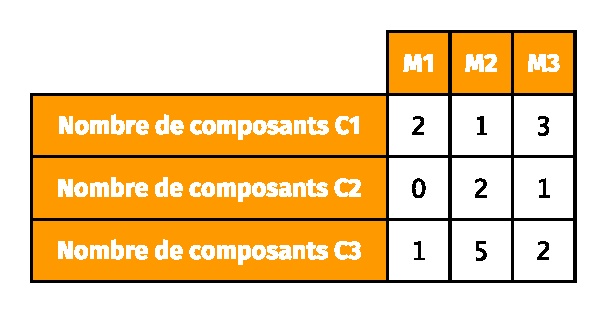
\includegraphics[width=8cm]{img/tableau}
\end{center}

Les prix et masses unitaires sont les suivants :

\begin{center}
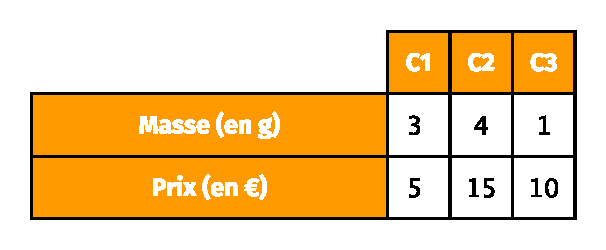
\includegraphics[width=8cm]{img/tableau2}
\end{center}

On note 
$A = \begin{pmatrix}
2&1&3\\
0 &2& 1\\
1 & 5 & 2
\end{pmatrix}$,
$B = \begin{pmatrix}
3&4&1\\
5&15&10
\end{pmatrix}$.\\

Calculer $B\times A$.\\

\carreauxseyes{16.8}{8}\\

On pose $C=B\times A$. Que représente $c_{12}$ ? Que représente $c_{23}$ ?\\

\carreauxseyes{16.8}{2.4}\\

Le directeur de l'usine souhaite fabriquer 10 matériels $M_1$, 20 $M_2$ et 30 $M_3$. On pose $C = \begin{pmatrix}
10\\20\\30
\end{pmatrix}$

Quelle opération matricielle permet d'obtenir le nombre de composants de chaque sorte pour réaliser les assemblages ? On ne demande pas d'effectuer l'opération.\\

\carreauxseyes{16.8}{2.4}


\end{document}

